%%% Document Author: J Moss
%%% Parts in LaTeX: Nicholas Dart
%%% Other Content: See authors list
%%% Document Last edit: 28.10.2014

\documentclass[11pt, article]{article}
\usepackage{a4wide}
\usepackage[english]{babel}
\usepackage{graphicx}
\usepackage{tabu}
\usepackage{textcomp}
\usepackage{fancyhdr}
\usepackage{lastpage}
\usepackage{titlesec}
\usepackage{lscape}
\usepackage{longtable}
\usepackage{color}
\usepackage{listings}
\usepackage{hyperref}

\definecolor{mygreen}{rgb}{0,0.6,0}
\definecolor{mygray}{rgb}{0.5,0.5,0.5}
\definecolor{mymauve}{rgb}{0.58,0,0.82}

\lstset{ % Syntax highliughting for java
    backgroundcolor=\color{white},   % choose the background color; you must add \usepackage{color} or \usepackage{xcolor}
    basicstyle=\footnotesize,        % the size of the fonts that are used for the code
    breakatwhitespace=false,         % sets if automatic breaks should only happen at whitespace
    breaklines=true,                 % sets automatic line breaking
    captionpos=b,                    % sets the caption-position to bottom
    commentstyle=\color{mygreen},    % comment style
    deletekeywords={...},            % if you want to delete keywords from the given language
    escapeinside={\%*}{*)},          % if you want to add LaTeX within your code
    extendedchars=true,              % lets you use non-ASCII characters; for 8-bits encodings only, does not work with UTF-8
    frame=none,                    % adds a frame around the code
    keepspaces=true,                 % keeps spaces in text, useful for keeping indentation of code (possibly needs columns=flexible)
    keywordstyle=\color{blue},       % keyword style
    language=Octave,                 % the language of the code
    morekeywords={*,...},            % if you want to add more keywords to the set
    numbers=left,                    % where to put the line-numbers; possible values are (none, left, right)
    numbersep=5pt,                   % how far the line-numbers are from the code
    numberstyle=\tiny\color{mygray}, % the style that is used for the line-numbers
    rulecolor=\color{black},         % if not set, the frame-color may be changed on line-breaks within not-black text (e.g. comments (green here))
    showspaces=false,                % show spaces everywhere adding particular underscores; it overrides 'showstringspaces'
    showstringspaces=false,          % underline spaces within strings only
    showtabs=false,                  % show tabs within strings adding particular underscores
    stepnumber=5,                    % the step between two line-numbers. If it's 1, each line will be numbered
    stringstyle=\color{mymauve},     % string literal style
    tabsize=4,                       % sets default tabsize to 2 spaces
    title=\lstname                   % show the filename of files included with \lstinputlisting; also try caption instead of title
}

%%%%%%
%% Variables for version and release status
%% useage: \version
%%%%%%
\newcommand\version{1.0}
\newcommand\release{Release}
\newcommand\titleText{Design Specification}
\newcommand\reference{SE\_O2\_DS\_00}

%%%%%%
%% Alias
%%%%%%
\newcommand{\sectionbreak}{\clearpage}  %% Allways start a section on a new page

\title{ \huge CS221 Group Project \\ \Large \titleText}
\author{
    \vspace{100pt}
    \begin{tabular}{ r || l }
        Project Team    &
            \begin{tabular}{l l}
                Aldridge, William & Atkins, Max \\
                Barnes, Alexander    & Dart, Nicholas \\
                Harizanov, Maksim & O'Hare, James \\
                Pocock, Michael   & Tuff, Sebastian \\
                Wilcock, Daniel   & Wilmot, Andrew \\
            \end{tabular} \\
        Version         & \version \\
        Status          & \release \\
        Date Published  & \today \\
        Reference       & \reference \\
        Department      & Computer Science \\
        Address         & Aberystwyth University \\
                        & Penglais Campas \\
                        & Ceredigion \\
                        & SY23 3DB \\
    \end{tabular} \\
    Copyright \textcopyright Aberystwyth University 2014
    %get rid of the date on the titlepage
    \date{}
}

\pagestyle{fancy}
\fancyhf{}
\rhead{Version \version~(\release)}
\rfoot{Page \thepage \hspace{1pt} of \pageref{LastPage}}
\lfoot{Aberystwyth University - Computer Science}

\begin{document}
    \setcounter{page}{1}

    \maketitle
    \thispagestyle{empty}

    \tableofcontents

    \section{Decomposition Description}
        \subsection{Subsystems}
	The Botanist Tools application is composed of 3 subsystems:
	\begin{itemize}
		\item Android Application
		\item Website
		\item Server
	\end{itemize}

	\subsubsection{Android Application}
		The android application provides the interface that users will use to record  plant data when out on a visit. It implements requirements (FR1), (FR2), (FR3), (FR4), (FR5), (FR6). It must also conform with the requirements (EIR1), (PR1),  (PR2), (DC1) and (DC2)~\cite{refSpec}.

		The application will have a form-based activity which can be used to add and edit new and currently saved recordings. Currently saved recordings will be stored locally in a collection, which will be awaiting dispatch to the server. The user will be able to view this list and select recordings to perform actions on (Eg. edit and delete). The application will not show recordings that are saved on the server. 

		The Android application will communicate with the server to perform functions such as sending recordings and performing user authentication. The application does NOT communicate directly with the website and the database. It uses a web API which is core to the server.

	\subsubsection{Server}

		The server will consist of two parts: 
		\begin{itemize}
			\item A database
			\item A web API
		\end{itemize}

	\subsubsection{Database}
		The database will be the central datastore for the entire system. It will communicate exclusively with the web API and serve as its back-end. 

	\subsubsection{Web API}
		The web API is central to the system; it provides a uniform way of accessing the database for all subsystems to use. It maintains the integrity of the datastore by acting as the ``middle-man'' so that the other subsystems do not damage the contents. It exposes a public interface to allow a set of actions to be performed by the users of the API; actions include user authentication and recordings management. The web API will implement the requirement (FR7) and must also conform to the requirement (PR2).

	\subsubsection{Website}
		The website will consist of a set of web-pages which implement all the required functionalities for the user (FR8) and (FR9). It must also conform to the requirements (EIR1), (PR1) and (PR2). The website will communicate with the Web API via HTTP to receive from and send data to the database. The website will have no communication with the Android application. It will also not directly communicate with the database, but will go through the web API. 


\subsection{Significant Android Components}

	\subsubsection{Significant UI classes}
		\begin{tabular}{r p{10cm}}
		HomeActivity & This class will hold the code to allow a user to move on to the NewRecordingActivity via a startNewRecordingButton. \\

		NewRecordingActivity & This class will hold the code to allow a user to enter information such as Name, Phone Number, E-Mail, and Site Location. It will also allow the application to receive date and time information from the Android device. The nextButton will then move the user to the AddNewSpeciesActivty. \\

		AddNewSpeciesActivity & This class will hold the code to allow a user to enter all the required information about a species entry in the current recording. It allows you to choose the name of a species from a locally saved list, and also allows the user to add a new species name, if not found. This activity must have the functionality to use the device's GPS capabilities to record location information of the species. It allows the user to select abundance in accordance with the DAFOR scale. The user should be able to add a scene/specimen picture through the device's camera or the gallery application. The user can also add a note if they wish. There is then a confirmButton which adds the species to the current recording and moves the user on to the MaintainRecordingActivity. \\

		MaintainRecordingActivity & This class will hold the code to allow a user to maintain the current recording. It will contain the functionality to edit any entered species from the collection in the recording. It will also allow the user to delete the current recording, removing all stored species data. The user will be able to save the recording, sending the current recording to the server at the first opportunity. \\
		\end{tabular}

	\subsection{Significant other classes}
		\begin{tabular}{r p{13cm}}
		Specimen & This class will hold the code to define all the information a specimen object can hold. Fields to hold this data will be: speciesName, gpsLocation, abundance, scenePicture, specimenPicture, notes. This class will also provide getter and setter methods for the mentioned fields.\\

		Recording & This class will hold the code to define all the information a recording object will hold. Fields to hold this data will be: usersName, usersPhoneNumber, usersEmail, usersAddress, dateTime. This class will contain getters and setters for the mentioned fields.\\
		\end{tabular}

\subsection{Significant Website Components}
	\begin{tabular}{r p{10cm}}
	Navigation & A set of buttons at the top of each webpage that will allow the user to move around the site. When clicking on the desired button, they will be taken to the designated page.\\

	Homepage & This landing page will provide all the general information a user needs to know about the service. It also contains a search bar which will allow the user to filter through the plant database to find what they are looking for. \\

	View Species Page & This page will display every species in the database for the user to view and select. If the user selects a species, they will be taken to the View Chosen Species Page, which provides more species information. This page will also allow the user to add a new species, taking them to the Add Species Page. \\

	View Chosen Species Page & This page will display all information about the specific species chosen by the user. \\

	Add Species Page & This page will provide all the forms necessary to input all data for a chosen species (name, location, abundance, scene picture, specimen pictures and notes), or allow a user to add a new species that is not listed. \\

	Map Overlay & This component will be a pop-up map that will show the locations of the chosen species. This location will be taken from the database.\\
	\end{tabular}

\clearpage
\subsection{Significant Server Components}

	\begin{tabular}{r p{10cm}}
	Server & A database and a set of Web API commands to allow manipulation. \\
	Database & a MySQL database where we will store all data for our system \\
		\begin{itemize}
			\item Tables 
			\begin{itemize}
				\item botany_users
				\item botany_records
				\item botany_specimens
				\item botany_reserves
				\item botany_resources
			\end{itemize}
		\end{itemize}
	Web API & A list of commands that allow the Android and website systems to access and manipulate data in the Database. \\
		\begin{itemize}
			\item addRecord.php - Adds a record to the database
			\item addReserve.php - Adds a reserve to the database
			\item addResource.php - Adds a resource (picture) to the database
			\item  authenticateAdmin.php - Checks an inputted password and tells if it's the same as the stored password
			\item getRecord.php - Returns a record 
			\item getRecords.php - Returns all records
			\item getReserve.php - Returns a reserve
			\item getReserves.php - Returns all reserves
			\item getResource.php - Returns a resource (picture)
			\item getSpecimen.php - Returns a specimen
			\item getSpecimens.php - Returns all specimens
			\item removeReserve.php - Removes a reserve
			\item removeSpecimen.php - Removes a specimen
			\item updateReserve.php - Updates a reserve
			\item updateSpecimen.php - Updates a specimen
		\end{itemize}

    \section{Android Application Design}
        \subsection{Decompisition}
	The compilation dependencies are as follows:
	\begin{itemize}
		\item Android dependencies a user will have an array of visits
		\item A visit will have an array of specimens
		\item A specimen can get data from the plant db (Fig \ref{fig:androidComponentDiagram}).
	\end{itemize}
	
	\begin{figure}
		\centering
			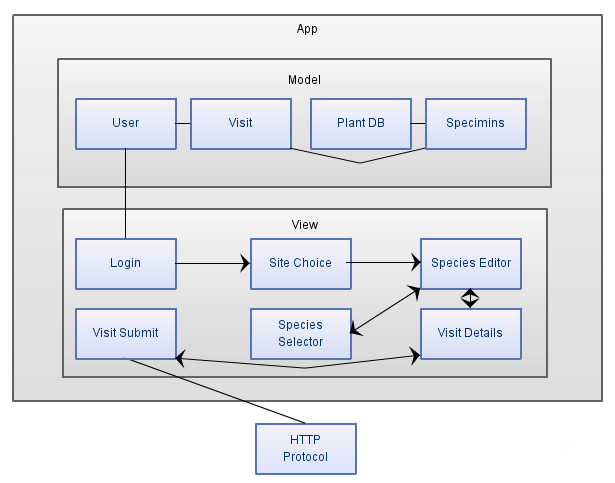
\includegraphics[scale=0.75]{android/componentDiagram.png}
		\caption{Component diagram for Android}
		\label{fig:androidComponentDiagram}
	\end{figure}

\newpage
\subsection{Interfaces}
	\subsubsection{Login Activity Interface}
		\lstinputlisting[language=Java, firstline=33]{android/src/loginInterface.java}

	\newpage
	\subsubsection{Site Choice Activity Interface}
		\lstinputlisting[language=Java, firstline=8]{android/src/siteChoiceInterface.java}

	\newpage
	\subsubsection{Species Selector Activity Interface}
		\lstinputlisting[language=Java, firstline=8]{android/src/speciesSelectorInterface.java}

	\newpage
	\subsubsection{Visit Management Activity Interface}
		\lstinputlisting[language=Java, firstline=8]{android/src/visitManagementInterface.java}

	\newpage
	\subsubsection{Visit Submit Activity Interface}
		\lstinputlisting[language=Java, firstline=8]{android/src/visitSubmitInterface.java}

	\newpage
	\subsubsection{User Data Class Interface}
		\lstinputlisting[language=Java, firstline=1]{android/src/userClassInterface.java}

	\subsubsection{Visit Data Class Interface}
		\lstinputlisting[language=Java, firstline=1]{android/src/visitClassInterface.java}

	\subsubsection{Plant DB Interface}
		This Will be a file obtained from the Botanical Society of Britain and Ireland containing a large list of known plant types in a comma sperated list (CSV) format. This file will be parsed at runtime and a condensed list created in alphabetical order for searching. Obtained from $http://www.bsbi.org.uk/resources.html$

	\subsubsection{Specimen Class Interface}
		\lstinputlisting[language=Java, firstline=1]{android/src/SpecimenClassInterface.java}


    \section{Web Design}
        \subsection{Interface}
<<<<<<< HEAD
	These are the server side scripts that will be used across the website.

	Constants
	\begin{itemize}
		\item Header
		\begin{itemize}
			\item session\_start();
			\item Doctype
			\item meta tags
			\begin{itemize}
				\item description
				\item Keywords
				\item authir
				\item content type
				\item CSS links
				\item Font link
				\item validation.js
				\item \$title
			\end{itemize}
			\item Header/Div
			\begin{itemize}
				\item Logo
			\end{itemize}
			\item /div
		\end{itemize}
		\item Nav
		\begin{itemize}
			\item Nav
			\item include`breadcrumbs';
		\end{itemize}
			
		\item Footer 
		\begin{itemize}
			\item Site map link 
			\item Icon
		\end{itemize}
			
		
		\item config.php
		\begin{itemize}
			\item \$host = `';
			\item \$port \= `';
			\item \$user \= `';
			\item \$password \= `';
			\item \$dbname \= `';
			\item mysql \= new mysql(\$...)
			\item die statements
		\end{itemize}

			
		\item Index
		\begin{itemize}
			\item \$title
			\item include `header.php';
			\item include `nav.php';
			\item text
			\item include `simple\_search.php';
			\item text
			\begin{itemize}
				\item app link
			\end{itemize}
			\item include `FOOTER';
		\end{itemize}
		\item plants
		\begin{itemize}
			\item include `config.php';
			\item \$title
			\item include `header.php';
			\item include `nav.php';
			\item add\_plant\_record link
			\item include `advanced\_search.php';
			\item include `plant\_db\_declare.php';
			\item include `plant\_sorting.php';
			\item include `footer.php';
		\end{itemize}

		\begin{itemize}
		\item add\_plants\_record
			\item include `config.php';
			\item \$title
			\item include `header.php';
			\item include `nav.php';
			\item form(input)  INSERT(SQL - add the form input into db)
			\item if no image uploaded, default image else uploaded image
			\item include `upload\_image.php';
			\item include `save\_record.php';
			\item a href `plants.php' cancel
			\item include `footer.php';
		\end{itemize}


		\item plants\_record
		\begin{itemize}
			\item include `config.php';
			\item \$title
			\item include `header.php';
			\item include `nav.php';
			\item \$specific record details
			\item a href `edit\_plant\_record.php' edit
			\item a href `delete\_plant\_record.php' remove
			\begin{itemize}
				\item delete prompt js
			\end{itemize}
			\item individual record photo or default image
			\item a href `plants.php' where to find
			\begin{itemize}
				\item (plant\_map.js)
			\end{itemize}
			\item include `footer.php';
		\end{itemize}		
			
		\item edit\_record
		\begin{itemize}
			\item include `config.php';
			\item \$title
			\item include `header.php';
			\item include `nav.php';
			\item include `breadcrumbs.php';
			\item \$individual record
			\item a href `edit\_plant\_record.php' edit
			\item a href `delete\_plant\_record.php' remove
			\item \$individual record photo
			\item a href `plants.php' where to find
			\begin{itemize}
				\item (plant\_map.js)
			\end{itemize}
			\item include `footer.php';
		\end{itemize}
	\end{itemize}
	
\subsection{Detailed design}
	\subsubsection{timeout.php}
		Time out is essentially a script that will unset a specific session when no activity has taken place, display and alert message, which once confirmed will send the user back to the plant list page. This will mainly be included when adding or editing records, as if the computer is left alone, then anyone could distort the record information.

	\subsubsection{plants.php}
		The plants page is where the list of plants are going to be displayed. The page will require the connection to the database through the config file, and it must include the html pages header.php, nav.php and the footer.php files.  The page will also have its own heading that will be created by a variable, will be declared above the header.php include, where the header will have \$title so it can be adjusted easily. The main content area below the navigation, which is then split into two. The first section is where the user will be able to sort the database records to their specific criteria. This sorting script will be placed in a separate file. The other half, is the main part of the page. In this section, the user can select a link that will allow them to create a new plant record and store it in the database. Under that, there is an advanced search, which will display records that comes under the criteria of their search input. This will also be in a separate script. This search will allow the user to not have to scroll through the long list of records. The plants are split into their scientific name and their common name. Once they are clicked, then they are taken to the plants individual record. The database itself is going to be called and declared from a separate script, where it will then place them into a table, which will present the plant lists.

	\subsubsection{db\_declare.php}
		This script is basically where and how the plant list will be created and how it will be represented. Firstly, the table will have to be created, which will have a div attached to it. Then the scientific and common headings will be created. Once this has been created, an SQL statement will be used, making a handle onto the database connection, where it will select all the fields by using.  We can then use the handle from the SQL statement to write out the database, using `while(\$row = pg\_fetch\_array (\$res))" and then defining the cells by calling them by \$row[`dbcolumn'] inside of td tags.  Each of these rows will be links to the page that has their information on. The table is then closed. The script does require config.php, but this is already included in plants.php

	\subsubsection{Plant location}
		When showing the specific location of the plant, we will be using the google maps JavaScript API. To use this we will have to gain an API key from google;once we have access, we must activate the Google Maps API v3. To get the API key, we must give it some information about the website, such as the web address. Because we will be testing it on another server, we will register it to that site first, which we can change to the server we will be using it on later on at the final part of the project.
	
		Implementing the code must start with giving the script source, included into the HTML head, where the API key must be inserted.  Then a new JavaScript script will be created, stating an initialize function. This will be made up of a variable mapProp, where it will specify all of the options for the map, such as where to center the map, how close are we going to zoom in on the location and what type of map is it going to be, such as Roadmap and Terrain, which we will be using HYBRID, as it allows to see a combination of the roads and the scenery, which may be useful to a botanist trying to find the specific plant. In these options however, is the lat/lang input, which will locate where the plant is. Because this depends on the location of the plant that will be displayed, we will have to use a variable that will get the latitude and longitude from the record and place it in the variable so it can there be used to display its location. After these options have been defined, the mapProp variable is closed, and the map is then created through creating a new map variable, which will assign itself to a div depending on its ID. The script must then be closed. To display this, in the body, there must be a div with the same ID stated in the script. 

	\subsubsection{config.php}
		config will open a link to the mysql database at the start of each new session, all changes to records and searches are reliant on this script.
		\begin{verbatim}
			\$conn = mysql\_connect("host=<localhost>
			port=3306 dbname=<nameofdatabase> 
			user=<uid> password=<password>");
		\end{verbatim}
		The script will also include a few lines closing the link to the database at the end of the session as not to produce more connections to the database than needed.

	\subsubsection{plant\_sorting.php}
		The plant data can be sorted in multiple different ways there will be a default sort using SORT\_REGULAR however the options of SORT\_STRING and SORT\_NUMERIC will also be available as required. The script will provide the user with an option of how they wish to sort the data.

	\subsubsection{simple\_search.php}
		The simple search script will search the database for a string matching the users input, all entries in the database containing that string will be returned. It will require a connection to the database from config.php, if there is no connection then the script will return an error message to notify the user of a problem with the connection to the database.

	\subsubsection{advanced\_search.php}
		The script for advanced search will allow for searches by string, ID, data type, location and user. The user should select their search type before inputting, the results shall be returned unless no result is found or there is an issue with the connection to the database in which case an error message shall be returned to the user. 

	\subsubsection{edit\_plant\_record.php}
		This script will take data input from the client side to form an update in an object oriented way. The update will set the field to be updated to the new data. The script will query if the connection to the server is valid before committing the changes, it will also return a confirmation to the user that the record has been updated or that there was a problem connecting to the server (they have timed out) so they can try again.

	\subsubsection{delete\_plant\_record.php}
		The script for deleting a record will be very straight forward, using an object oriented approach the script will request for the record to be deleted by using its ID. Much like the edit this script will return a confirmation to the user that the record has successfully been deleted or that there was a problem with the connection to the server.

	\subsubsection{upload\_image.php}
		This script should prompt the user to choose an image file to upload first, when an image file has been selected an upload function will collect the data about the file where it can be validated to check it matches the requirements we have set (eg: file type and size). The image file, if compatible, will be uploaded and the script will return a success message, otherwise a message will be returned to the user explaining which parameter is incorrect or if there is an issue with the connection to the server.

	\subsubsection{regex validation}
		validation will be done on the client side using javascript and regular expressions. Doing this allows us to use an onchange method when the user is inputting data with fixed parameters, such as what characters can be used, without putting extra load on the server.


    \section{Server Design}
        \subsection{Interface}
    These are the commands that the web API will be using to maintain the database and receive commands.
    \begin{itemize}
        \item AddRecord
        \item Headers required:
        \begin{itemize}
            \item none
        \end{itemize}
        \item POST arguments:
        \begin{itemize}
            \item record : Record
        \end{itemize}
        \item Statuses:
        \begin{itemize}
        	\item 200 OK:
            \begin{itemize}
        		\item record ID : Integer
            \end{itemize}
        	\item 400 Bad Request
        	\item 500 Internal Server Error
        \end{itemize}

        \item RemoveRecord
        \item Headers required: 
        \begin{itemize}
        	\item Authorization
        \end{itemize}
        \item POST Arguments:
        \begin{itemize}
        	\item recordID : Integer
        \end{itemize}
        \item Statuses:
        \begin{itemize}
        	\item 200 OK : no data
        	\item 400 Bad Request
        	\item 401 Unauthorized
        	\item 500 Internal Server Error
        \end{itemize}

        \item ModifyRecord
        \item Headers required:
        \begin{itemize}
        	\item Authorization
        \end{itemize}
        \item POST Arguments:
        \begin{itemize}
        	\item recordID : Integer
        	\item record : Record
        \end{itemize}
        \item Statuses:
        \begin{itemize}
        	\item 200 OK : no data
        	\item 400 Bad Request
        	\item 401 Unauthorized
        	\item 500 Internal Server Error
        \end{itemize}


        \item GetRecord
        \item Headers required: 
        \begin{itemize}
            \item none
        \end{itemize}
        \item POST Arguments:
        \begin{itemize}
        	\item recordID : Integer
        \end{itemize}
        \item Statuses:
        \begin{itemize}
        	\item 200 OK :
            \begin{itemize}
                \item record : Record
            \end{itemize}
        	\item 400 Bad Request
        	\item 500 Internal Server Error
        \end{itemize}

        \item GetRecords
        \item Headers Required:
        \begin{itemize}
        	\item none
        \end{itemize}
        \item POST Arguments:
        \begin{itemize}
            \item maxResultCount : Integer
            \item resultStartOffset : Integer?
        	\item speciesFilter : String?
            \item abundanceFilter : Integer?
            \item userNameFilter : String?
            \item fullNameFilter : String?
            \item commentFilter : String?
            \item locationNameFilter : String?
            \item locationLatitudeProximityFilter : Float?
            \item locationLongitudeProximityFilter : Float?
            \item locationProximityRadius : Float?
        \end{itemize}
        \item Statuses: 
        \begin{itemize}
        	\item 200 OK : array of Record
        	\item 400 Bad Request
        	\item 500 Internal Server Error
        \end{itemize}

        \item AddResource
        \item Headers required: 
        \begin{itemize}
            \item none
        \end{itemize}
        \item POST Arguments:
        \begin{itemize}
        	\item resource : OctetStream
        \end{itemize}
        \item Statuses:
        \begin{itemize}
        	\item 200 OK :
            \begin{itemize}
        		\item resource ID : Integer
            \end{itemize}
        	\item 400 Bad Request
        	\item 500 Internal Server Error
        \end{itemize}

        \item GetResource
        \item Headers required:
        \begin{itemize}
            \item none
        \end{itemize}
        \item POST Arguments:
        \begin{itemize}
        	\item resourceID : Integer
        \end{itemize}
        \item Statuses:
        \begin{itemize}
        	\item 200 OK : 
            \begin{itemize}
                \item resource data : OctetStream
            \end{itemize}
        	\item 400 Bad Request
        	\item 500 Internal Server Error
        \end{itemize}
    \end{itemize}

\subsection{Detailed design}
    \subsubsection{Diagrams}
        \begin{figure}
            \centering
            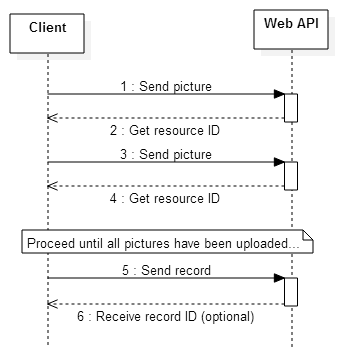
\includegraphics[scale=0.75]{server/working/SequenceDiagram-AddRecord.png}
            \caption{Sequence diagram: adding a record through the web API}
            \label{fig:addRecordSequenceDiagram}
        \end{figure}

        \begin{landscape}
            \begin{figure}
                \centering
                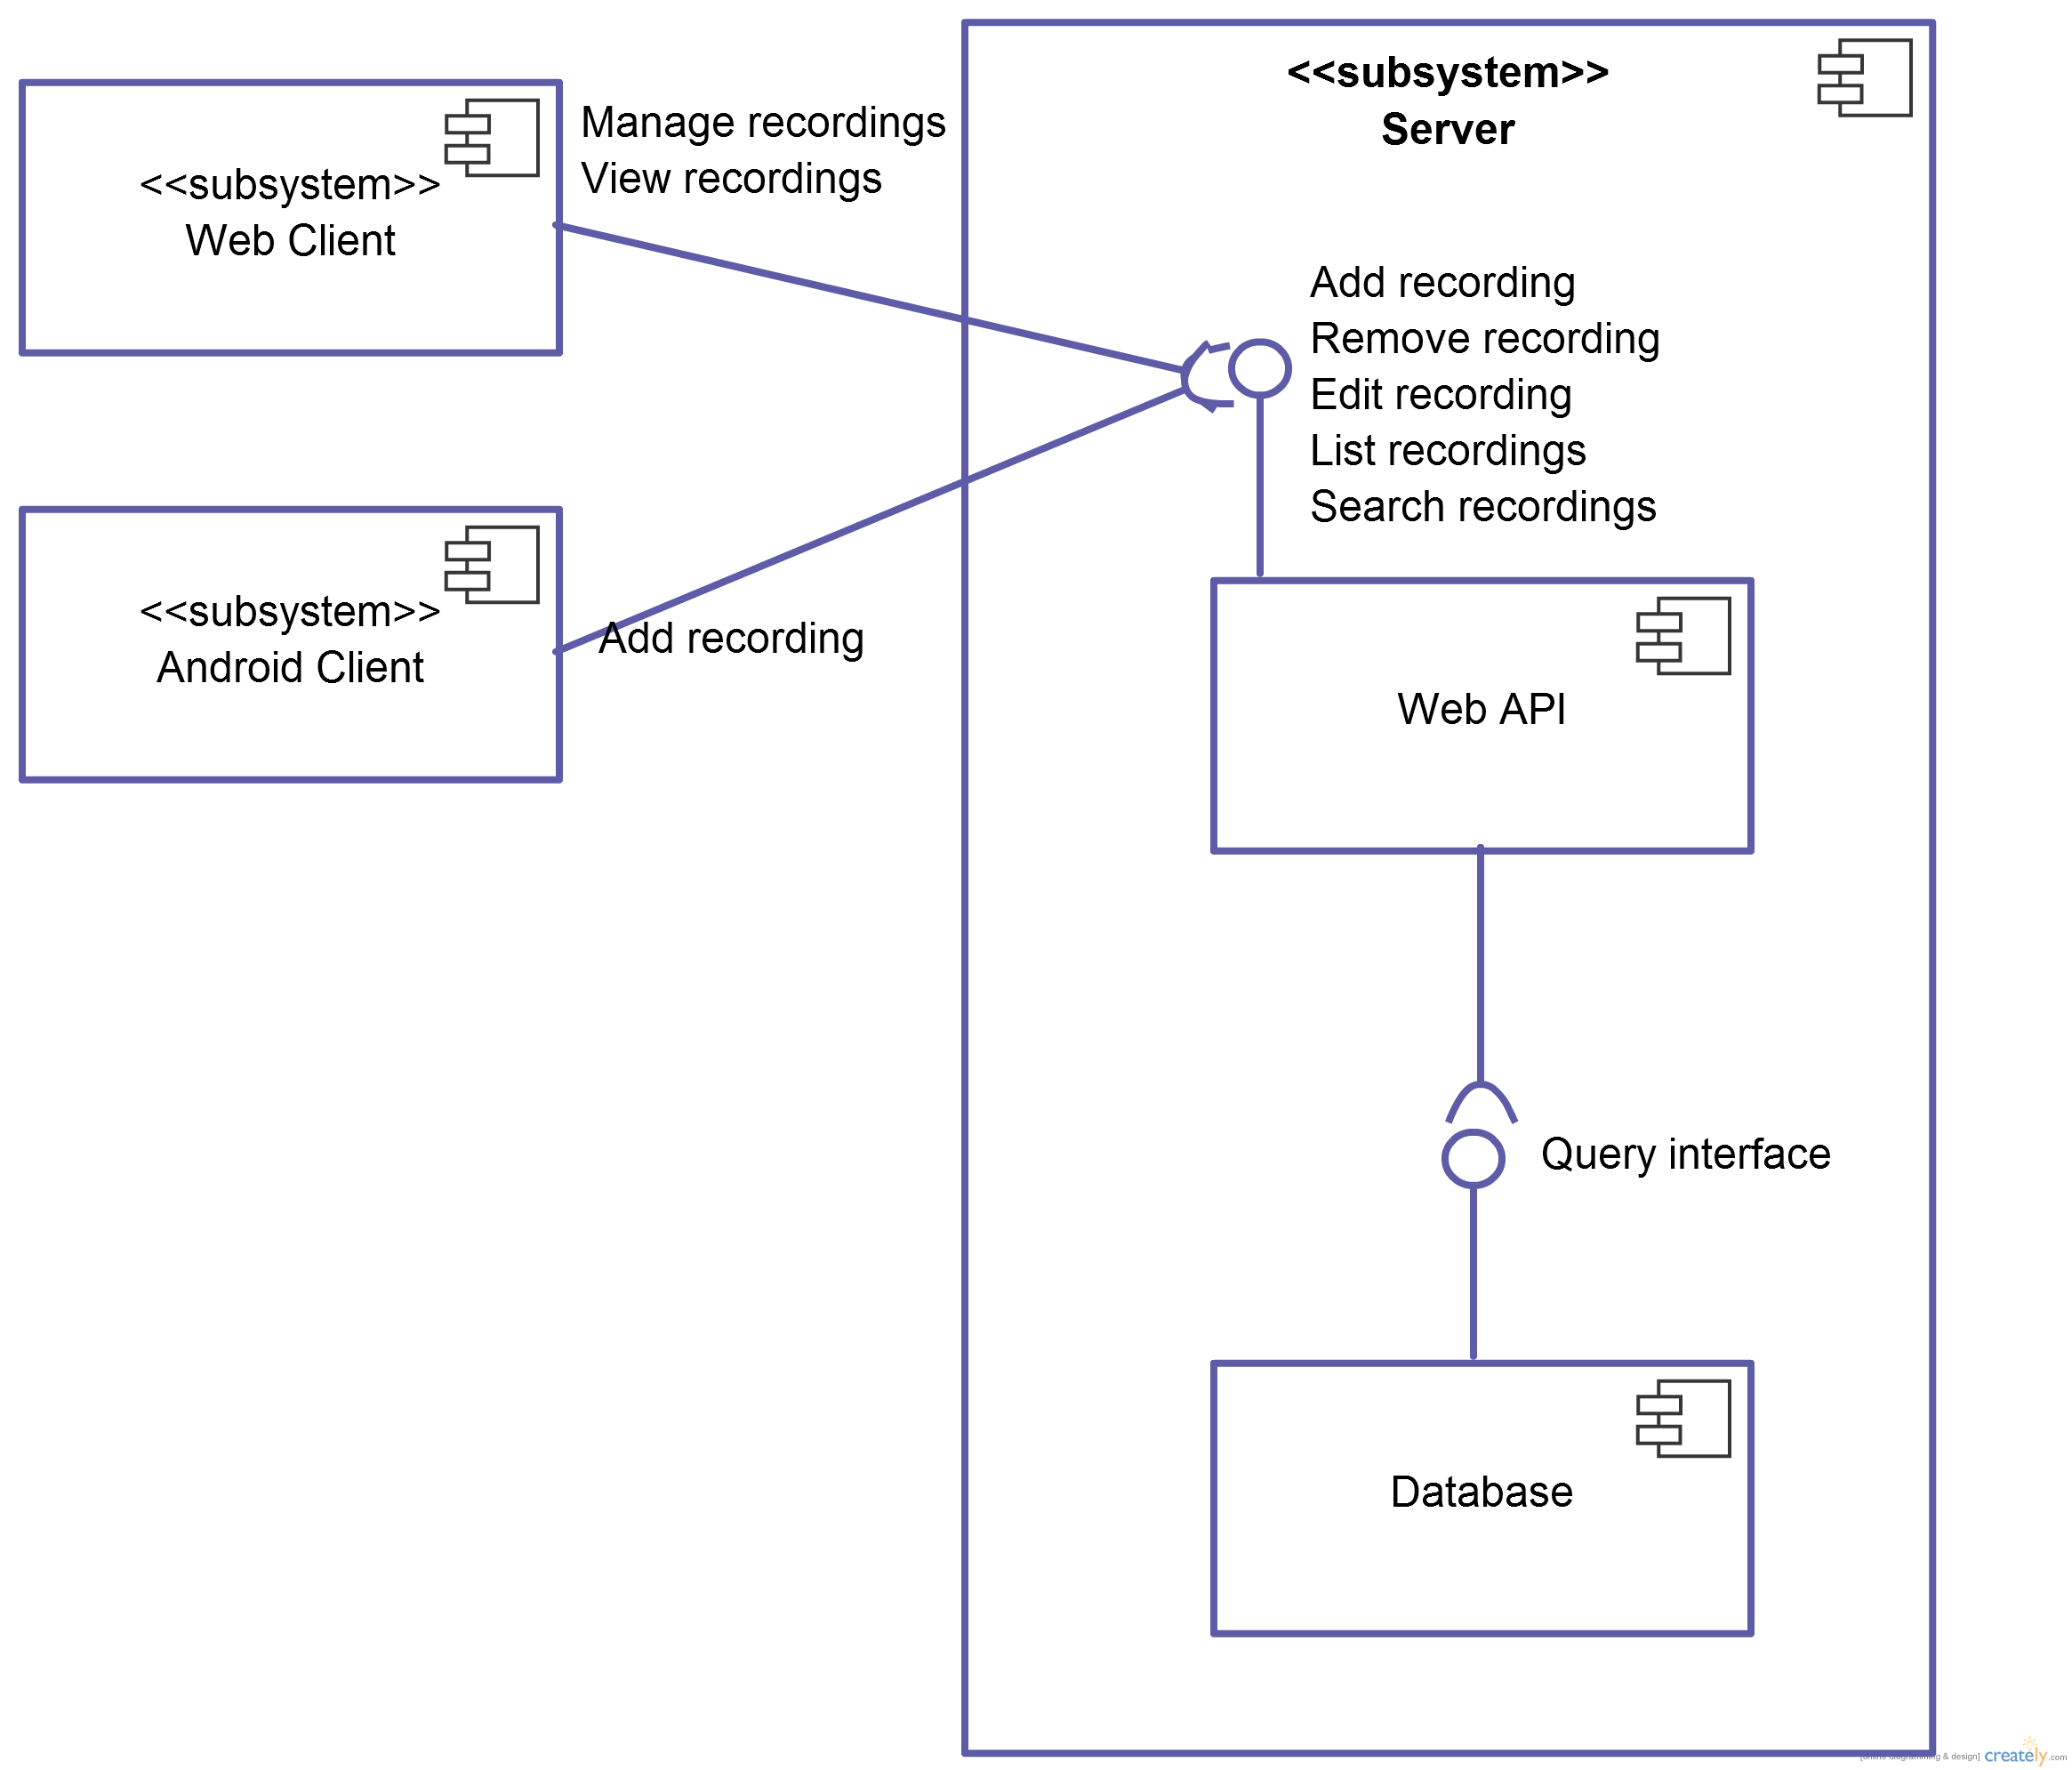
\includegraphics[scale=0.2]{server/ComponentDiagram.png}
                \caption{Web Api component Diagram}
                \label{fig:webAPIComponentDiagram}
            \end{figure}
        \end{landscape}

    \subsubsection{Significant data structures}

        The web API is going to make use of the Record and Specimen data structures, which will be exchanged between the server and its clients (the Android application and the website). They will be represented in a JSON format, which is readily available for use in PHP, JavaScript, and Android. Data types, where specified, are JSON data types. 

        The structure of a Record is as follows:
        \begin{itemize}
            \item Record : Object
            \begin{itemize}
                \item UserName : String
                \item UserPhone : String
								\item UserEmail : String
                \item LocationName : String 
                \item Specimens : Array of Specimen
            \end{itemize}
        \end{itemize}

        The structure of a Specimen is as follows:
        \begin{itemize}
            \item Specimen : Object
            \begin{itemize}
                \item SpeciesName : String
                \item LocationLatitude : Number
                \item LocationLongtitude : Number
                \item Abundance : Number
                \item Comment : String
                \item ScenePhoto : String (ID of a resource on the server)
                \item SpecimenPhoto : String (ID of a resource on the server)
            \end{itemize}
        \end{itemize}

        The web API is going to use a relational database as a data store.
        The database tables are as follows:

        \begin{itemize}
            \item Users
            \begin{itemize}
                \item UserId : INT auto-increment PK
                \item UserName : VARCHAR(20) not-null
                \item UserFullName : VARCHAR(50)
                \item UserPhone : VARCHAR(20)
                \item UserEmail : VARCHAR(50)
                \item UserPassword : BINARY(20)
            \end{itemize}
                
            \item Records
            \begin{itemize}
                \item RecordId : INT auto-increment PK
                \item UserId : INT not-null
                \item LocationName : VARCHAR(50)
                \item Timestamp : INT
            \end{itemize}
                
            \item Resources
            \begin{itemize}
                \item ResourceId : INT auto-increment PK
            \end{itemize}

            \item Specimens
            \begin{itemize}
                \item SpecimenId : INT auto-increment PK
                \item RecordId : INT not-null
                \item SpeciesName : VARCHAR(255) not-null
                \item Latitude : FLOAT(10,6)
                \item Longitude : FLOAT(10,6)
                \item Abundance : INT
                \item Comment : TEXT
                \item ScenePhoto : INT
                \item SpecimenPhoto : INT   
            \end{itemize}
        \end{itemize}

    \begin{thebibliography}{9}
        \bibitem{refSpec} Project Plan Specification Standards :B. P. Tiddeman (2014-09-23) SE.QA.05b 1.2
    \end{thebibliography}

    \section{Document History}
        \begin{tabular}{l || p{8cm} | l | r}
            Version & Edit & Date & Persons \\ \hline 
            0.1 & Initial Version & November 5 2014 & nid21 \\ \hline
            0.2 & Updated with decomposition description & November 12 2014 & nid21 \\
            0.3 & Updated with Android interfaces & November 17 2014 & nid21 \\
            0.4 & Included web and server sections & November 27 2014 & nid21 \\
            0.5 & Document review & November 28 2014 & nid21 \\
            0.6 & More document reviewing and preparing for release & December 02 2014 & nid21 \\
            0.7 & Updated web design spec & Febuary 11 2015 & jao14 \\
        \end{tabular}

\end{document}
